\documentclass[10pt, a4paper]{article}

\usepackage[top=1cm, bottom=1cm, left=1cm, right=1cm]{geometry}
\usepackage{titling}
\usepackage{graphicx}
\usepackage{url}
\usepackage{wrapfig}
\usepackage{algorithm}
\usepackage{algorithmic}
%\usepackage{algpseudocode}

\setlength{\droptitle}{-6em} 
\title{\scshape{\underline{Our project report}}}
\author{Rebekah Stephens- C1330222, Timothy Standen- C1323632,\\ Rosie Sproule- C1306213, Anna Johnson- C1370910}
\date{15 Febuary, 2014}
\bibliographystyle{plain}
\begin{document}
\maketitle
\begin{wrapfigure}{R}{35mm}
	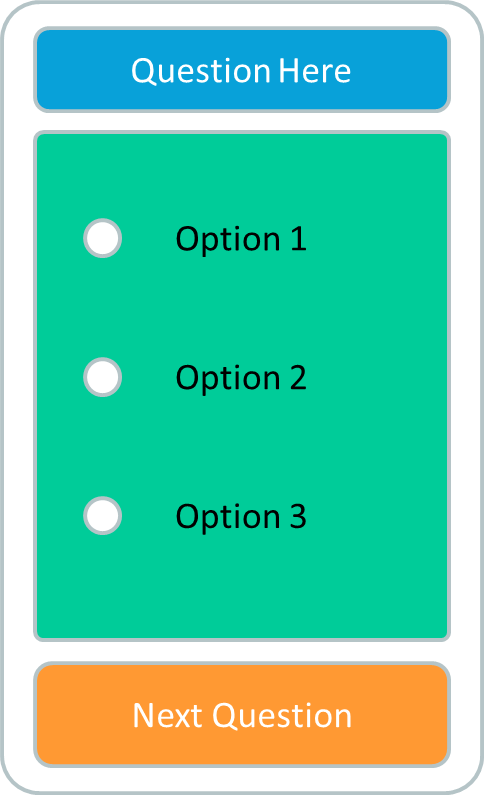
\includegraphics[width = 28mm]{images/Picture8.png}
	\label{muiltquestion}
	\caption{Sample design of Q\&A page.}
\end{wrapfigure}
\section{Product definition}


We have noticed an upcoming opportunity of a gap in the market and decided to produce a Mathematical online self-learning application.The difference to our competitors is that we are aiming to an older generation 16+, we're not linking to the school curriculum and also we're going for a "want to learn" approach rather than a school enforced learning system. \\
To promote the application before the launch, we are going to create a website to show what the application is, what the app will include, pricing, expectation and pre-ordering. \\\\
The process of making the app will include some multiple choice quiz's as shown in Figure \ref{muiltquestion} in which the user would answer, and their result would be saved. The questions are going to be stored in a file, such that the same general code can be applied for all code, with the difference being the quiz id.
\begin{verbatim}
CurrentQuestion <-- 1
CorrectAnswers <-- 0
Repeat
    Question <-- Questionfile[QuizID][CurrentQuestion][0]
    Option 1 <-- Questionfile[QuizID][CurrentQuestion][1]
    Option 2 <-- Questionfile[QuizID][CurrentQuestion][2]
    Option 3 <-- Questionfile[QuizID][CurrentQuestion][3]
    Update labels for Quesion, Option 1, Option 2 and Option 3 on screen
    Wait for user to press submit
    if CheckOption = Questionfile[QuizID][CurrentQuestion][4] then
        CorrectAnswers <-- CorrectAnswers + 1
    CurrentQuestion <-- CurrentQuestion + 1
Until CurrentQuestion = LastQuestion

print CorrectAnswers
\end{verbatim}
\section{Market Research}
To begin with, we wanted to see our competitors and what they were offering. From the results of this, we could plan how to differ from other leading brands.\\
In Figure \ref{Appstore} are the math applications, that are already on the market;
\begin{figure}[H]
	\begin{center}
		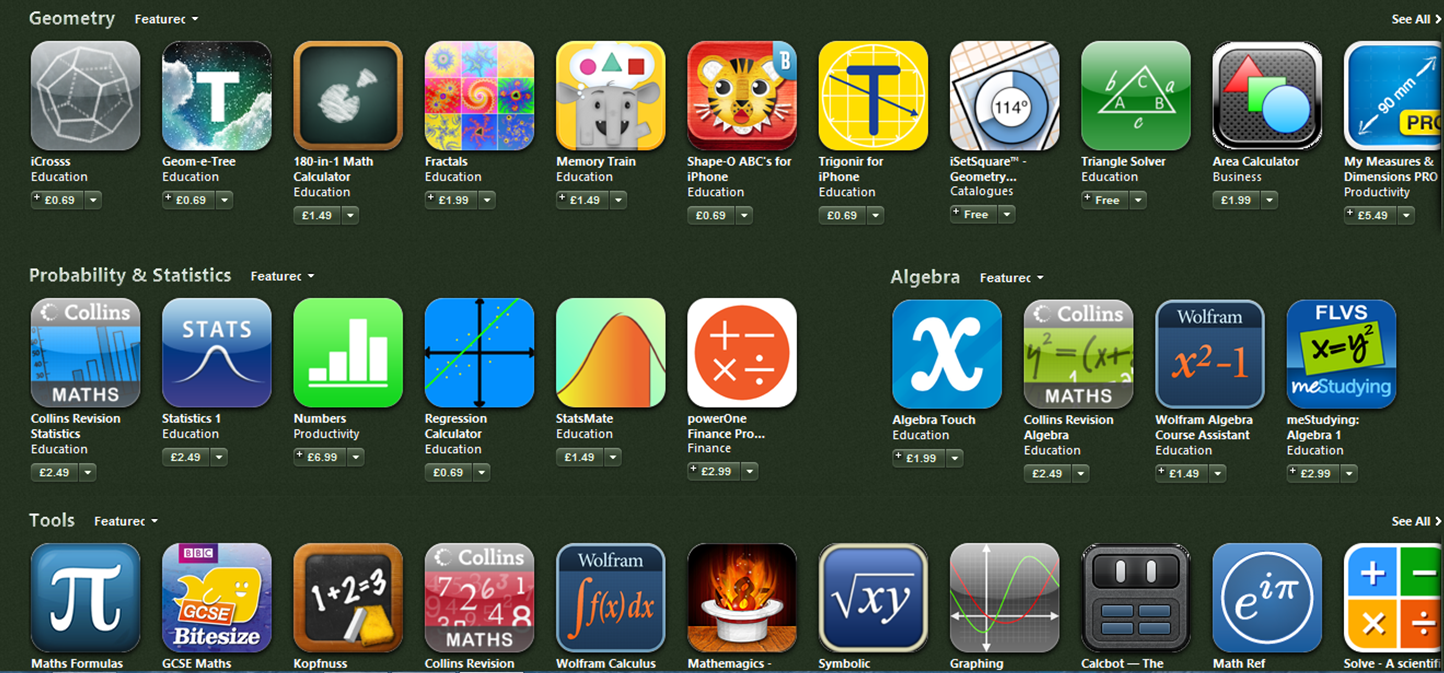
\includegraphics[height= 7.5cm]{images/Picture5.png}
		\caption{Current Apps as shown on the from the app store in iTunes. \cite{appstore}}
		\label{Appstore}
	\end{center}
\end{figure}
\underline{Points to consider:}
\begin{itemize}
	\item General prices = £0.69, £1.49, £1.99, £2.49 or free.
	\item Neutral colour schemes: greens, blues, oranges, colour that stand out against each other.
	\item Maybe if they've got the answer wrong either show them how to do it clearly, or show them the topic area in which they could find the help.
	\item Achievement badges?
	\item Login shouldn't be connected to a hotmail, facebook, googlemail etc.
	\item Shouldn't need internet/wifi to open or use (like some games).
	\item Could have several versions of apps e.g. geometry, calculus etc...
	\item Clear easy layout for all ages.
	\item Available points to collect to work towards a badge/certificate?
	\item Needs to be versatile for not only apple but window products.
	\item Should be applicable to apple products over younger iOS generations and have update button for when the new iPod/iPhone/iPad versions come out.
\end{itemize}

Here are some examples of our existing competitors:

\begin{minipage}{0.45\textwidth}
\underline{Applications}

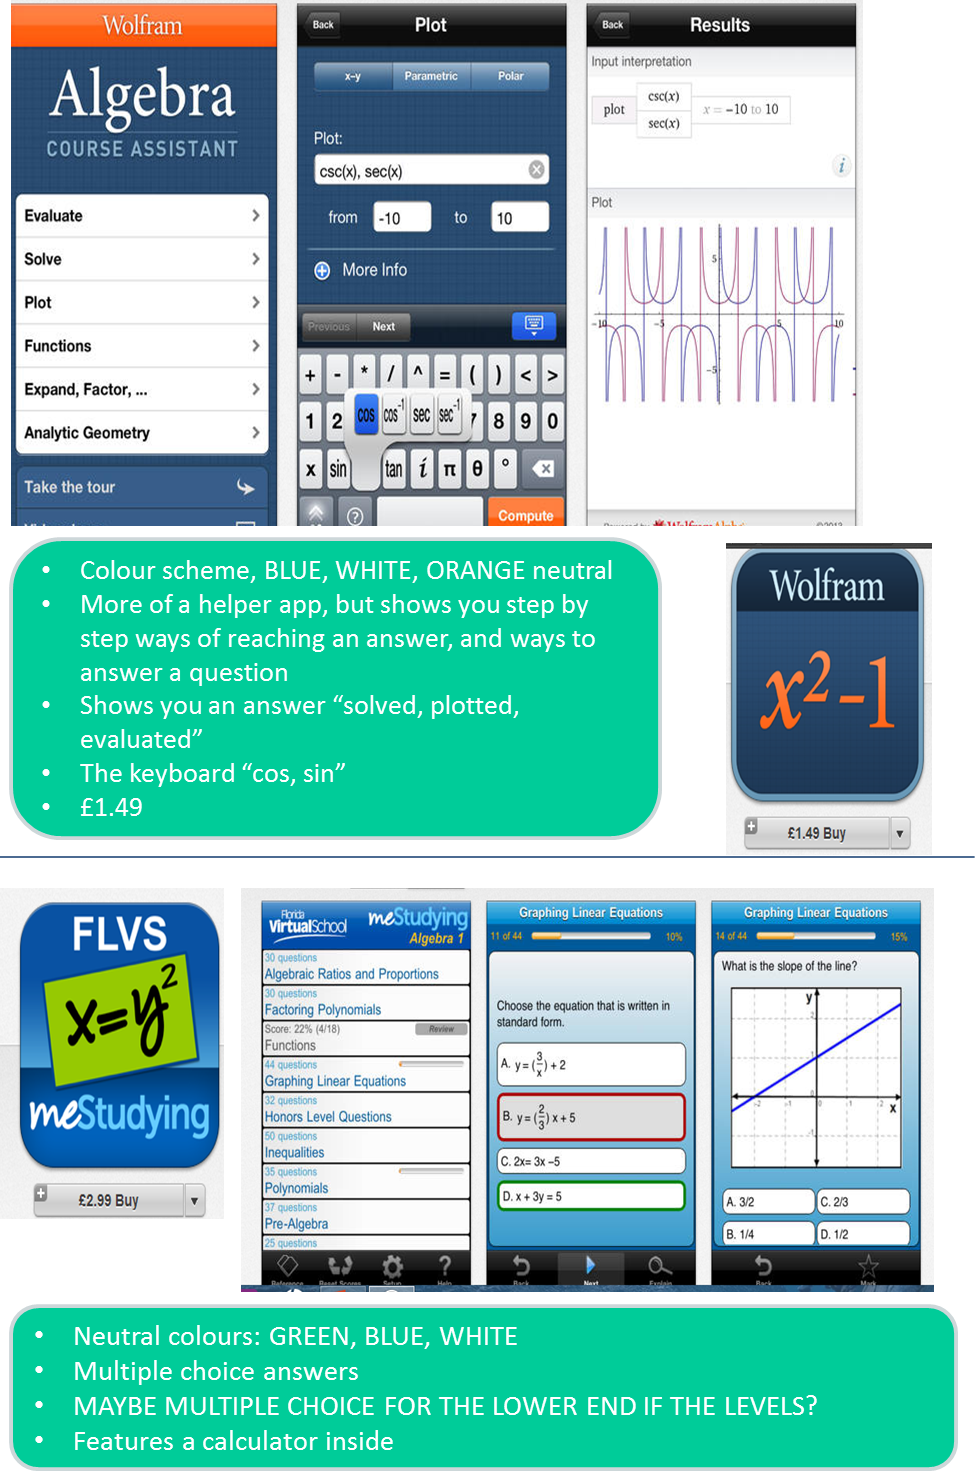
\includegraphics[width=80mm, height=120mm, keepaspectratio = true]{images/Picture4.png}
\end{minipage}
\hfill
\begin{minipage}{0.45\textwidth}
\underline{Websites}

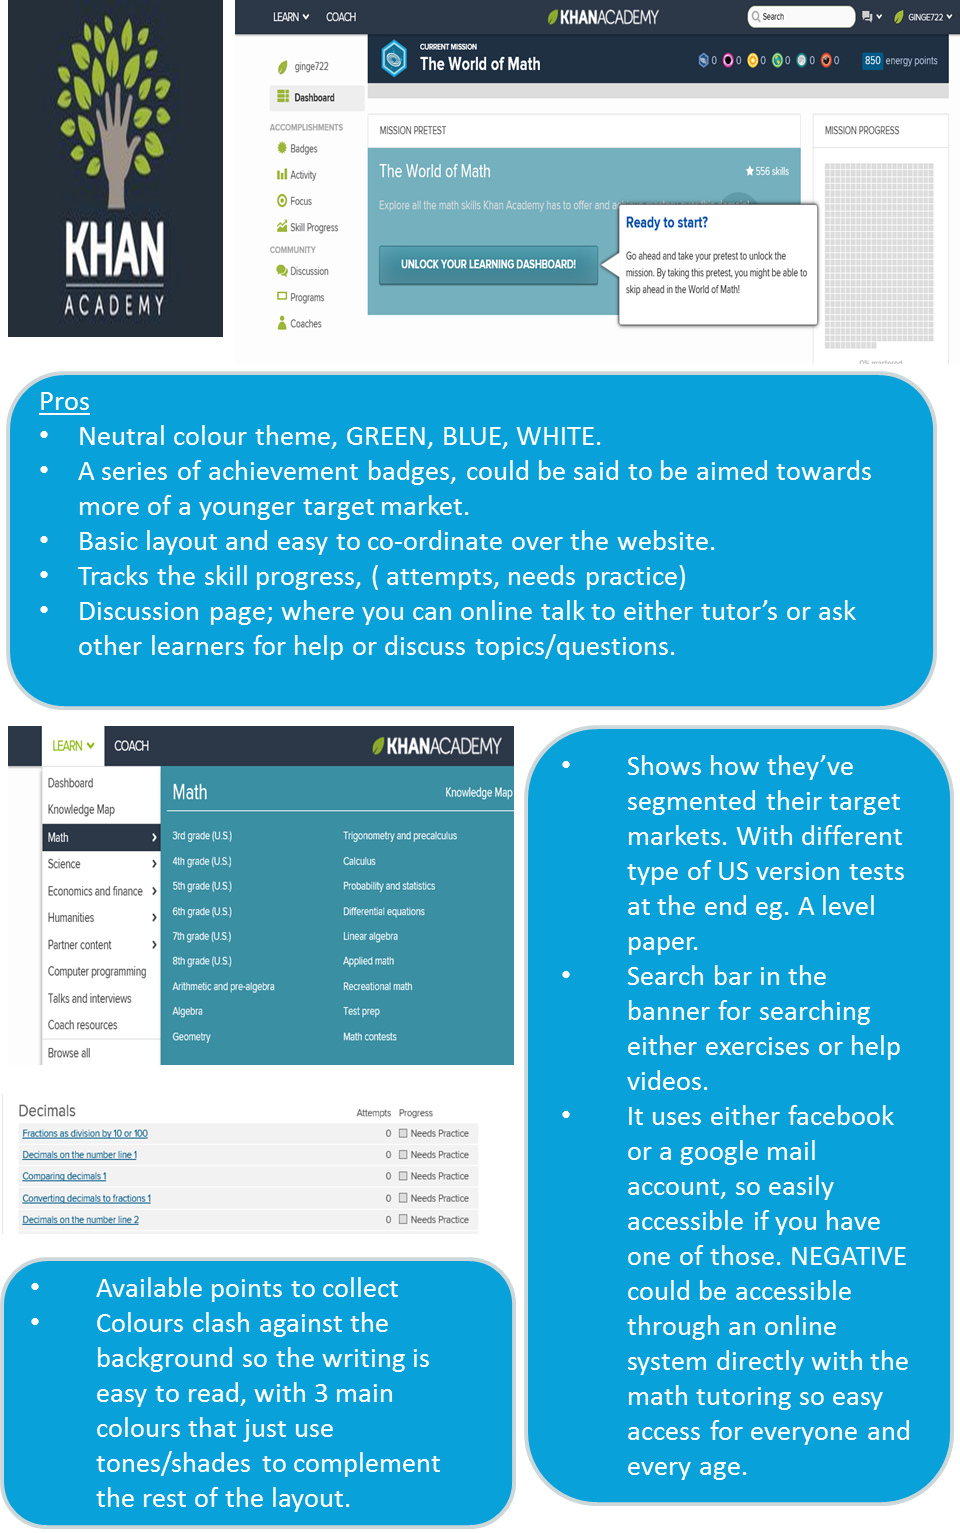
\includegraphics[width=80mm, height=120mm, keepaspectratio = true]{images/Picture6.png}
\end{minipage}

\section{Strategy}
To plan our strategy we broke it down into 6 key and vital areas. \\
\begin{itemize}
	\item Promotion
	\item Branding
	\item Price
	\item Product 
	\item Research
	\item Place
\end{itemize}

\begin{figure}[H]
	\begin{center}
		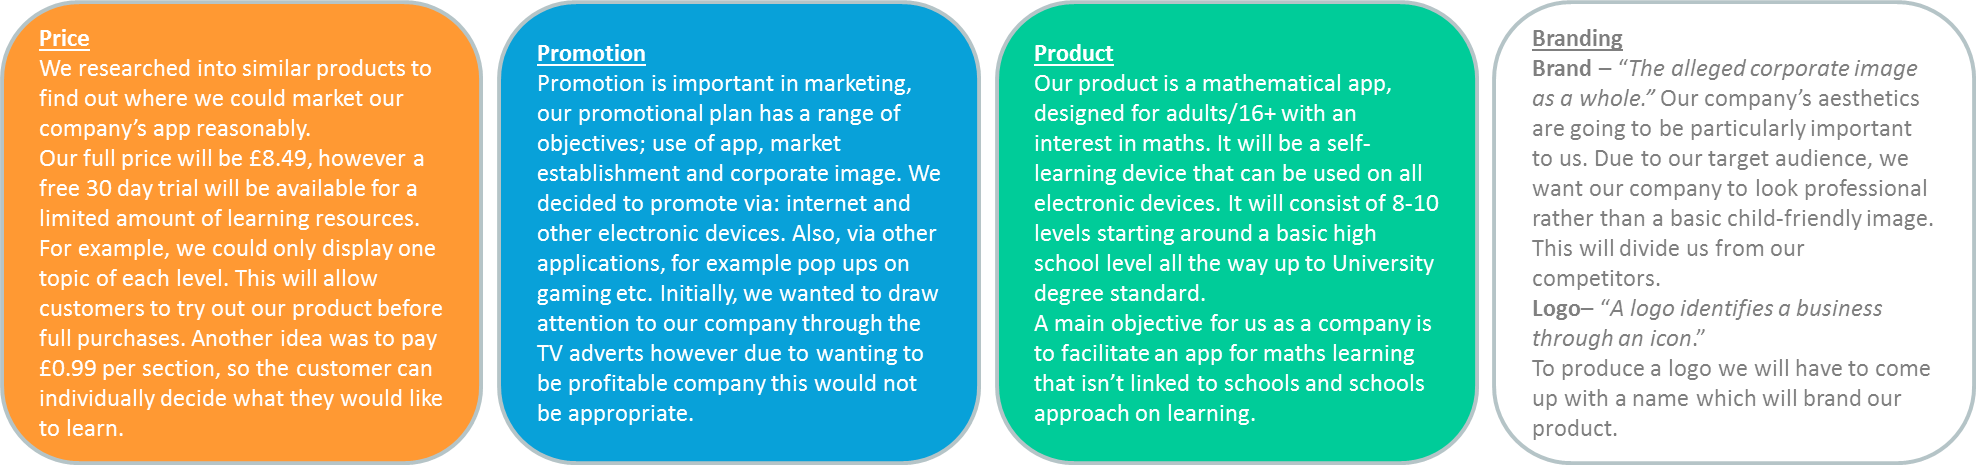
\includegraphics[width=190mm]{images/Picture7.png}
		\caption{Definitions for brand and logo are from \cite{brandinglogo}}
	\end{center}
\end{figure}

The mediums of which we can promote and advertise our product are as follows;\\

\begin{tabular}{| p{1.5cm} | p{5cm} | p{5cm} | p{5cm} |}
	\hline
	Medium & Advantages & Disadvantages & Cost \\
    \hline
    Television & Mass market covered, powerful response, can include sound. & Target market chosen by time its aired, quick/limited exposure & Expensive, especially for peak viewing times. \\
    \hline
	Magazines & Good coverage on chosen area, accepted, high quality photos. & Short exposure time, no guarantee on positioning. & High cost in national magazines and positions. \\
    \hline
	Billboard & Positioned in high traffic areas, flexible, repeated exposure & Can't chose audience fully, potentially vandalised & Low cost but can be expensive dependent on location. \\
    \hline
	Internet & Instant, can be virtual, direct, popular, high exposure. & Linked to spam, not everyone used the internet yet. & Low cost and product can be bought over the internet. \\
    \hline
\end{tabular}
\\\\
By looking at the advantages and disadvantages we came to the conclusion that the best way of promoting our product would be, in fact by making a "branded" website.\\\\
We decided upon the colour scheme in Figure \ref{colours} for our website and application, we feel that this would give us a professional looking product whilst still being aesthetically pleasing to the eye.
\begin{figure}[!h]
	\begin{center}
		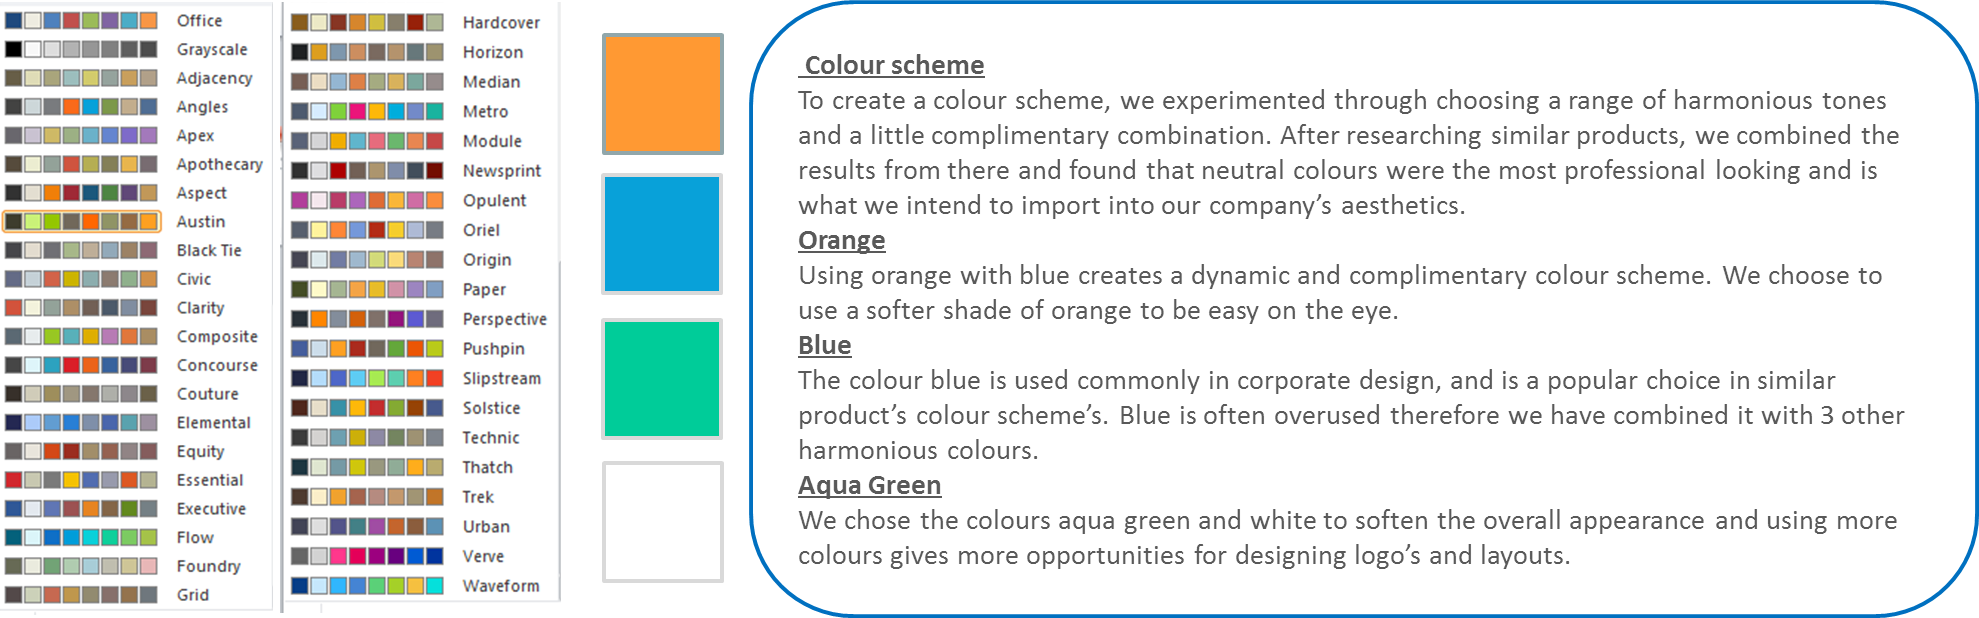
\includegraphics[width=19cm]{images/Picture3.png}
		\caption{Different colours themes options in PowerPoint \cite{powerpointcolours}, and our chosen colour scheme.}
		\label{colours}
	\end{center}
\end{figure}

\bibliography{bibliography.bib}

\end{document}